\chapter{Grundlagen}

\section{Digitale Plattformen als disruptive Innovation}

\subsection{Definition und begriffliche Abgrenzung}

Gegenwärtig sind sowohl in der wissenschaftlichen Literatur als auch in der unternehmerischen Praxis zahlreiche unterschiedliche Definitionen zur Kategorisierung von digitalen Plattformen vorhanden. Diese haben gemeinsam, dass sie grundsätzlich zwischen einer marktorientierten und einer technologieorientierten Betrachtungsperspektive unterscheiden, welche in einem komplementären Bezug zueinanderstehen und sich somit ergänzen. \footnote{\cites[Vgl.][S. 21-23]{ENGELS2017}; \cites[Vgl.][S.99]{MEINHARDT2019}}
%\autocite[Vgl.][S. 21-23]{ENGELS2017} \autocite[Vgl.][S.99]{MEINHARDT2019}



Aus einem \textbf{technologieorientierten Blickwinkel} wird eine digitale Plattform als eine Menge von Kernprodukten, -technologien oder -services verstanden, auf deren Basis weitere komplementäre Produkte, Technologien oder Services entwickelt und angebunden werden können.\autocite[Vgl.][S. 21]{ENGELS2017} Folglich werden hier auch komplexe Informations- technologie-Systeme (\acsu{it}-Systeme), Software- und Hardware-Plattformen dazugezählt.\autocite[Vgl.][S.222f]{WEINREICH2016}

Aus einer \textbf{marktorientierten Perspektive} wird eine Plattform als ein Markt betrachtet, in welchem gegenseitige Nutzerinteraktionen zu Netzwerkeffekten führen. \autocite[Vgl.][S. 1273f]{EISENMANN2011} Diese sind aufgrund der digitalen Plattform mit minimalen Investitionen skalierbar, weshalb sie insbesondere in traditionellen Märkten als disruptive Innovation angesehen werden. \autocite[Vgl.][S. 17ff]{MOAZED2016} Hierbei begünstigen die technologischen Möglichkeiten wie Cloud-Computing in Verbindung mit den Netzwerkeffekten die Bildung von Oligopol- bzw. Monopol-Marktstrukturen.\autocite[Vgl.][S. 23]{ENGELS2017} Ein Beispiel hierfür sind die sogenannten \acsu{gafa} Unternehmen: Google (Alphabet), Apple, Facebook (Meta) und Amazon, welche digitale Plattformen zur Realisierung von digitalen Ökosystemen einsetzen und sich dadurch ihre führende Marktposition sichern konnten. \autocite[Vgl.][S. 92f]{BUNTE2020} 
%\improvement{Bernd: Aufbauen bereits bei Realisierung impliziert}

Nach dem Frauenhofer \ac{iese} ist ein digitales Ökosystem ein sozio-technisches System, bei dem Menschen und Unternehmen über eine digitale Plattform zusammenzuarbeiten, um eine Wertschöpfung zu erzielen, welche ohne das Ökosystem nicht möglich wäre. \autocite[Vgl.][S. 376]{MULLERSTEWENS2019} Dabei stellt die digitale Plattform die technologische Grundlage für das dazugehörige Ökosystem dar. \autocite[Vgl.][S. 376]{IESE2021} Folglich sind die beiden Termini sehr eng miteinander verknüpft.

Für die Untersuchung dieser Arbeit werden digitale Plattformen nach dem technologieorientierten Perspektive definiert. Diese wird in Kapitel \ref{sec:TechPCloud} noch weiter erläutert. 

%Im Rahmen dieser Arbeit soll die Einsatzmöglichkeiten SAP \ac{btp} bei deutschen \ac{kfz}-Versicherern evaluiert werden, weshalb in der Analyse dieser Arbeit digitale Plattformen nach dem technologieorientierten Ansatz definiert werden. Diese werden in Kapitel \ref{sec:TechPCloud} noch weiter erläutert. 

%weshalb insbesondere die technische Betrachtungsweise für die Arbeit relevant ist. Diese wird in ... mit Cloud Computing auf technischen Plattformen noch weiter erläutert.

\subsection{Wertschöpfung digitaler Plattformen}

Bei der Betrachtung der Wertschöpfung muss neben der digitalen Plattform als solches auch das dazugehörige Ökosystem betrachtet werden, in welchem die Plattform die Koordinationsstruktur für die unterschiedlichen Teilnehmer darstellt. Die digitale Plattform ermöglicht das gemeinsame Wertschöpfen, auch Value Co-Creation genannt, durch die Bereitstellung von komplementären Services und Produkten. Dabei ist der Wert der Plattform von den in Wechselwirkungen stehenden Faktoren der Größe des Kundenstamms als auch von der Vielfältigkeit der angebotenen Produkte und Services abhängig. Diese bestehende Wechselwirkung wird umgangssprachlich auch als „chicken and egg dilemma“ bezeichnet und stellt eine besondere Herausforderung für neu entstehende digitale Plattformen dar, weil keine der beiden Seiten bereit ist, sich anzuschließen, solange die andere Partei nicht ausreichend vertreten ist. \autocite[Vgl.][S. 310]{CAILLAUD2003} 
%\improvement{Liest sich kacke, versteht Luca nicht} 
Diese Wechselwirkung führt zu den sogenannten Netzwerkeffekten, welche vor allem mit einer steigenden Anzahl an Teilnehmern exponentiell zunehmen. Daher haben sowohl Plattformbetreiber als auch Kunden und Partner ein großes Interesse möglichst viele potenzielle Nutzer auf die Plattform zu bringen und mit ihnen zu interagieren. \autocite[Vgl.][S. 596f.]{HAHN2016} 

Die Wertschöpfung digitaler Plattformen wird auch durch das Schaffen neuer Vertriebskanäle unterstützt. So werden traditionelle Vertriebsstrukturen durch elektronische Marktplätze ersetzt und dadurch der Kundenzugang für komplementäre Dienstleister erleichtert. Diese profitieren darüber hinaus auch von vereinfachten und vereinheitlichten Transaktions- und Koordinationsaktivitäten. Dies kann beispielsweise durch die Standardisierung von Prozessen und Informationsflüssen erfolgen. So sind Applikationen für den Endkunden bereits vor integriert, können bei Bedarf schnell erworben und produktiv genutzt werden.\autocite[Vgl.][S. 599f.]{HAHN2016}

Des Weiteren ergeben sich aus Sicht des Plattformbetreibers ebenfalls Mechanismen zur Wertabschöpfung durch Bundling und durch den Lock-in-Effekt. Bundling bezeichnet den Verkauf von gebündelten Produkten und Dienstleistungen für einen vorher bestimmten Preis. Abhängig vom Preismodell können diese entweder zu einem festen Preis erworben oder bis zum produktiven Nutzen in einem Freemium Model kostenlos getestet werden.\autocite[Vgl.][S. 178-185]{TEECE2010} Der Lock-in-Effekt beschreibt die Tendenz von Nutzern und Partnern aufgrund hoher Wechselkosten und mangelnder Interoperabilität langfristig an eine bestimme Plattform gebunden zu sein. \autocite[Vgl.][S. 22]{STEUR2022} Er wird in der Praxis vor allem durch proprietäre Technologie oder das strategische Platzieren von Produkten und Dienstleistungen erreicht. \autocite[Vgl.][S. 704]{BALLON2011}

Um dieser Bedrohung zu entgehen, können Kunden und Partner auf mehreren konkurrierenden Plattformen vertreten sein und damit das sogenannte Multihoming betreiben. \autocite[Vgl.][S. 461ff]{CENNAMO2018} Zudem profitieren Kunden von der Modularität digitaler Plattformen, welche entlehnt aus der Systemtheorie, die Zerlegung komplexer Systeme in separate Subsysteme (Module) bezeichnet, die jeweils alle autark funktionieren. \autocite[Vgl.][S. 2]{LECHNER2019} Folglich können Kunden selbst entscheiden, welche Funktionen und Services sie von der Plattform nutzen möchten.


%\subsection{Cloud-Computing auf digitalen Plattformen}
\subsection{Cloud-Computing auf technologischen Plattformen}\label{sec:TechPCloud}
%Cloud Computing bei einer technologischen Betrachtungsweise von Plattformen)

\
Die Bereitstellung und Nutzung von Software und Hardware als Service hat sich als langfristiger Trend sowohl im Verbraucher- als auch im Geschäftskundensegment etabliert und ist mittlerweile unter dem Schlagwort \enquote{Cloud-Computing} allgegenwärtig. Eine einheitliche Definition dieses Begriffs ist in der Wirtschaft und Wissenschaft bisher nicht vorhanden. Allerdings haben die meisten Definitionen Überschneidungspunkte, welche in der Beschreibung des \ac{nist} zusammengefasst werden: 

\begin{center}
    \textit{\enquote{Cloud-Computing ist ein Modell für den allgegenwärtigen und bedarfsgerechten Netzzugang zu einem gemeinsam genutzten Pool konfigurierbarer Rechenressourcen (z. B. Netze, Server, Speicher, Anwendungen und Dienste), die mit minimalem Managementaufwand oder geringer Serviceprovider-Interaktion zur Verfügung gestellt werden können.}} \autocite[S. 2]{MELL2011}
\end{center}

Dabei wird Cloud Computing in drei verschiedene Servicemodelle \ac{iaas}, \ac{paas} und \ac{saas} unterteilt. Während bei \ac{iaas} Hardware-Ressourcen wie Server, Netzwerke, Middleware und Speicherplatz bereitgestellt und vom Nutzer selbst verwaltet werden können, sind es bei \ac{saas} die Software-Applikationen, die der Anwender über das Netz nutzt. Die dazugehörigen Verwaltungsaufgaben der genutzten Cloud Infrastruktur werden bei \ac{saas} vom Anbieter durchgeführt. Im Kontext digitaler Plattformen sind insbesondere \ac{paas}-Lösungen relevant.\autocite[Vgl.][S. 2f]{MELL2011} Diese stellen ein Set an Technologien zum Betreiben und Entwickeln von \ac{saas}-Applikationen bereit und übernehmen für den Nutzer die Verwaltung der Infrastruktur.\autocite[Vgl.][S. 8]{BRAUNINGER2012}

Die Hauptkomponente von \ac{paas} Lösungen ist die \ac{are}, welche als Ausführungsumgebung für \ac{saas}-Applikationen dient und die üblichen Anforderungen an Cloud-Software wie zum Beispiel Mandantenfähigkeit, Skalierbarkeit und Verfügbarkeit erfüllen muss. Eine \ac{are} ermöglicht dabei häufig eine Multi-Tenancy-Architektur, damit mehrere Nutzer eine Instanz einer \ac{saas}-Applikation nutzen können. Darüber hinaus wird eine integrierte Entwicklungsumgebung (\acs{ide}) bereitgestellt, welche mehrere Programmiersprachen unterstützt und Entwicklern verschiedene Bibliotheken sowie Werkzeuge zum Modellieren, Implementieren und Testen bietet. Abhängig von der Anwendungsdomäne können unterschiedliche Datenbankensysteme unterstützt und zusätzlich auch externe Datenquellen über \acp{api} integriert werden. \autocite[Vgl.][S. 371]{BEIMBORN2011}

Zunehmend werden zudem auf \ac{paas}-Lösungen auch Services zur Datenverarbeitung und Datenanalyse, Dienste zur Anbindung von \ac{iot} Geräten als auch eine Reihe von Tools zur Entwicklung von \ac{iot}-Anwendungen zur Verfügung gestellt. \autocite[Vgl.][]{IBM2023}

Darüber hinaus lassen sich \ac{paas}-Angebote auch in Bezug auf das Vorhandensein von sogenannten \ac{saas}-Kern-Applikationen unterscheiden. Es gibt reine \ac{paas}-Angebote wie beispielsweise die Google App Engine. Zusätzlich gibt es jedoch auch von großen Softwareherstellern betriebene \ac{paas}-Lösungen auf Applikationsbasis \acsu{apaas}, auf denen Entwickler Erweiterungen für eine \ac{saas}-Applikation entwickeln und dabei auf Daten und Funktionen der Kernapplikation zugreifen können. Ein Beispiel hier ist die von \ac{paas} von Salesforce Force.com mit der Kernapplikation Salesforce.com, bei der die Erweiterung ausschließlich als Ergänzung zur Kern-Applikation sinnvoll sind. \autocite[Vgl.][S. 371]{BEIMBORN2011} 

Neben den bisher dargestellten Komponenten stellen Plattformbetreiber häufig weitere Dienste entlang der Wertschöpfungskette bereit, wie beispielsweise Marketing und Vertrieb über elektronische Marktplätze. Weitere Mehrwertdienste umfassen hier ebenfalls die Abwicklung von Transaktionen und Zahlungen, einschließlich Aktivitäten wie Vertragsabschluss, Rechnungsstellung und regelmäßiger Zahlungsabwicklung. Des Weiteren können Support-Dienstleistungen wie First-Level-Support, Zertifizierung, Qualitätssicherung sowie Monitoring Funktionalitäten angeboten werden. \autocite[Vgl.][S. 598]{HAHN2016} Eine Übersicht über die obligatorischen und optionalen Komponenten einer \ac{paas} Lösung ist in Abbildung \ref{fig:PaaSK} dargestellt.

%\autocite[Vgl.][S. 599]{HAHN2016}
%\autocite[Vgl.][S. 372]{BEIMBORN2011}

\begin{figure}[h]
    \centering
    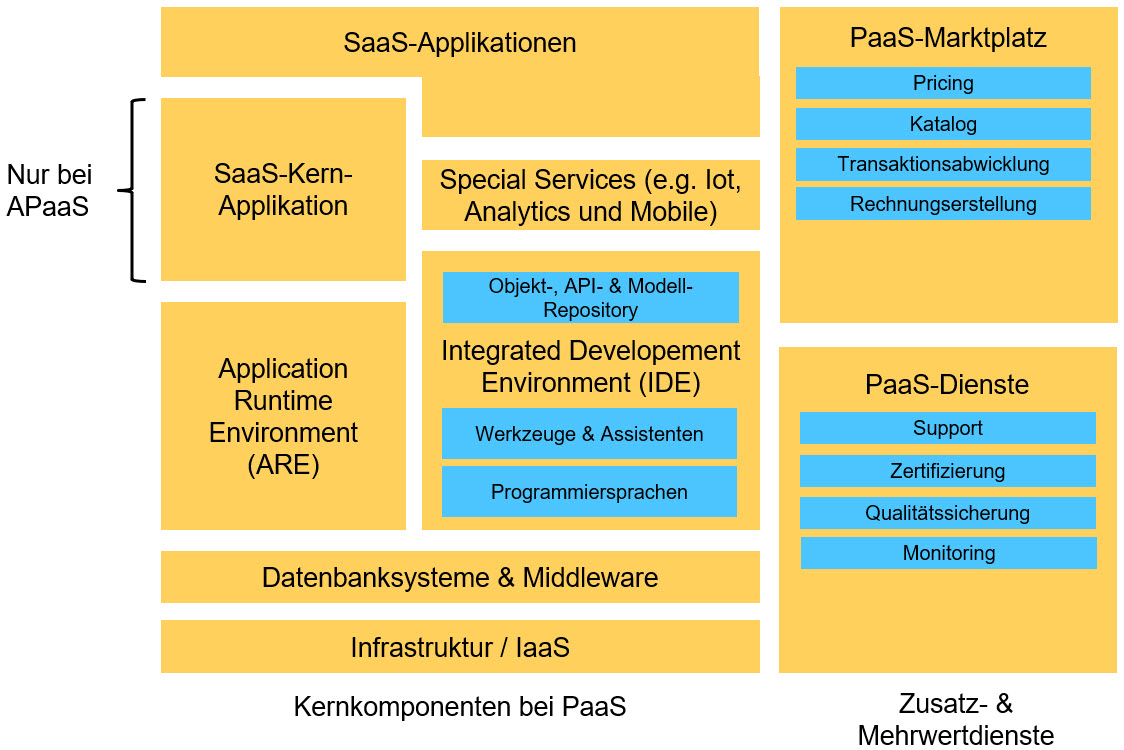
\includegraphics[width=0.9\textwidth]{img/PaaS_Komponenten.jpg}
    \caption[Komponenten einer PaaS-Lösung]{Komponenten einer PaaS-Lösung\autocite{PaaSK}}
    \label{fig:PaaSK}
\end{figure}
\footnotetext{Vgl. eigene Darstellung angelehnt an: Hahn, 2016, S. 599 und Beimborn et al., 2011, S. 372.}

%\improvement{Grafik anpassen --> SaaS Applikation kann ja wohl kaum verpflichtend sein, wenn ich PaaS kaufe}

In einem solchen Plattform-Ökosystem gibt es mindestens drei Akteure: Den Plattformbetreiber, die Komplementäre, welche beispielsweise Entwickler oder auch ein \ac{isv} Entwickler sein können, sowie die Endkunden. Der Plattformbetreiber stellt im Falle von \ac{apaas} die Plattform mit der dazugehörigen Kernapplikation zur Verfügung und ermöglicht es Komplementären wie \ac{isv}s Add-Ons für sein Kernprodukt zu entwickeln, um die Reichweite des Hauptproduktes zu steigern. Die \ac{isv} können zur Entwicklung von Erweiterungen und Stand-alone-Applikationen dabei auch bestehende Teile der Plattform nutzen und neu kombinieren. Darüber hinaus kann der Plattformanbieter auch selbst die Rolle eines Anwendungsentwicklers einnehmen.\autocite[Vgl.][S. 444f]{FOERDERER2018} Für den Endkunden selbst ist häufig nicht erkennbar, von wem die Applikation erstellt wurde, da er diese im Sinne des \ac{saas} direkt vom \ac{paas}-Anbieter bezieht. \autocite[Vgl.][S. 372]{BEIMBORN2011}

\subsection{SAP Business Technology Platform}

Die SAP Business Technology Platform ist eine cloudbasierte Technologieplattform, die es Unternehmen ermöglicht, Anwendungen zu erstellen, zu integrieren, zu verwalten und zu skalieren. Die Plattform wurde erstmals im Mai 2020 auf der SAPPHIRE-NOW Konferenz vorgestellt und zuvor als SAP Cloud Platform vertrieben, mit einem Fokus auf Applikationsentwicklung und Integration.\autocite[Vgl.][S. 2]{PREUSS2021}  Aktuell lassen sich die bereitgestellten Funktionalitäten der SAP \ac{btp} in die fünf Bereiche Datenmanagement, Datenanalyse, Anwendungsentwicklung, Integration sowie intelligente Technologien unterteilen. Als \ac{apaas}-Lösung umfasst die SAP \ac{btp} in den einzelnen Bereichen nicht nur eine, sondern mehrere Kernapplikationen, wie beispielsweise bei der Datenanalyse mit den Anwendungen SAP Analytics Cloud und SAP Data Warehouse Cloud. Die Services sind dabei modular miteinander kombinierbar und werden hauptsächlich über \ac{iaas}-Dienste bereitgestellt. Hierbei werden im Rahmen der 4 + 1 Multi-Cloud Strategie der SAP die Rechenzentren der Anbieter Amazon Web Services, Google Cloud, Microsoft Azure, Alibaba sowie SAP unterstützt. Dadurch stehen die Funktionen der Plattform in mehreren Rechenzentren weltweit zur Verfügung und erlauben eine globale Umsetzung der Anwendungsszenarien.\autocite[Vgl.][S. 57-59]{SEUBERT} Eine umfassende Beschreibung der fünf Funktionsbereiche der SAP \ac{btp} ist Kapitel \ref{sec:TechCharak} zu entnehmen.

\improvement{SAP Data Warehou Cloud später nicht erwähnt}

%\improvement{Noch Abbildung zu den Bausteinen der SAP BTP}

\section{Die deutsche Versicherungsbranche}

\subsection{Definition und Grundprinzipien der Versicherung}

Aufgrund der kontinuierlichen Weiterentwicklung des Versicherungsmarktes und der wachsenden Teilnahme unterschiedlicher Wirtschaftsdisziplinen an der Versicherungswissenschaft gibt es heutzutage eine Vielzahl von Definitionen für den Begriff der Versicherung. Bei Fokussierung auf die ökonomischen Aspekte wird in der Literatur insbesondere auf den Wirtschaftswissenschaftler Prof. Dr. Dieter Farny verwiesen, welcher das Versicherungsprodukt, auch Versicherung oder Police genannt, definiert als die: 

\begin{center}
    \textit{\enquote{Deckung eines im Einzelnen ungewissen, insgesamt geschätzten Mittelbedarfs auf der Grundlage des Risikoausgleichs im Kollektiv und in der Zeit.}} \autocite[S. 8f.]{FARNY2011}
\end{center}

Folglich ist die Versicherung ein Produkt zur Deckung von Sicherheitsbedürfnissen, indem es Risiken auf eine Gefahrengemeinschaft, das Kollektiv, überträgt. Die Befriedigung dieser Sicherheitsbedürfnisse umfassen die Absicherung von materiellen als auch beruflichen Risiken und sind auf der zweiten Ebene der Maslowschen Bedürfnispyramide zu finden. \autocite[Vgl.][S. 30]{BECKER2019} Das zugrunde liegende Konzept wird als Risikotransfer bezeichnet, bei dem der Versicherungsnehmer gegen Zahlung einer Prämie das Risiko auf den Versicherer überträgt. Beim Eintreten eines entsprechenden Schadens, dem Versicherungsfall, erhält der Versicherungsnehmer von der Versicherung einen Schadensausgleich. Dieser Risikoausgleichseffekt wird von Versicherungsunternehmen genutzt, um die systematische Übernahme von Risiken mit einem im Hinblick auf die Gewinnmöglichkeiten akzeptablen unternehmerischen Risiko durchzuführen. \autocite[Vgl.][S. 9]{FARNY2011}
Grundvoraussetzung ist hierbei, dass der Umfang der Schäden statistisch abschätzbar und dadurch der benötigte Beitrag jedes Mitglieds des Kollektivs mathematisch bestimmbar ist. Aufgrund dieser Kombinationen von Risikotransfer und Prämienzahlung werden Versicherungsunternehmen auch als Finanz- und Risikointermediäre bezeichnet. \autocite[Vgl.][S. 53]{ZWACK2017}

Grundsätzlich wird zwischen zwei Arten von Versicherungsunternehmen unterschieden: Erstversicherer und Rückversicherer. Erstere schließen ausschließlich Versicherungsgeschäfte mit gewerblichen Unternehmen, privaten und öffentlichen Haushalten ab, währenddessen Rückversicherer das daraus resultierende Risiko der Erstversicherer übernehmen.\autocite[Vgl.][S. 240f.]{FARNY2011} 
%\improvement{beachten, dass nicht über den Rand steht}

Darüber hinaus sind deutsche Erstversicherer durch verschiedene regulatorische Anforderungen wie dem \ac{vag} und der \enquote{Solvency II}-Richtlinie der Europäischen Union verpflichtet, um die Stabilität und Integrität des Versicherungsmarktes zu wahren. \autocite[Vgl.][]{BAFIN2016} Eine der fundamentalen Vorschriften ist die Spartentrennung nach § 6 II \ac{vag}. Demnach müssen Erstversicherungsunternehmen getrennte Geschäftsbereiche für Lebens-, Kranken- und Kompositversicherungen führen. Zur Gruppe der Kompositversicherungen, welche auch als Schaden- und Unfallversicherung bezeichnet wird, zählen seit dem 30.06.1990 alle Versicherungen, die nicht zur Lebens- und Krankenversicherung gehören und damit auch die \ac{kfz}-Versicherung. \autocite[Vgl.][S. 241-243]{FARNY2011} 

\begin{figure}[h]
  \centering
    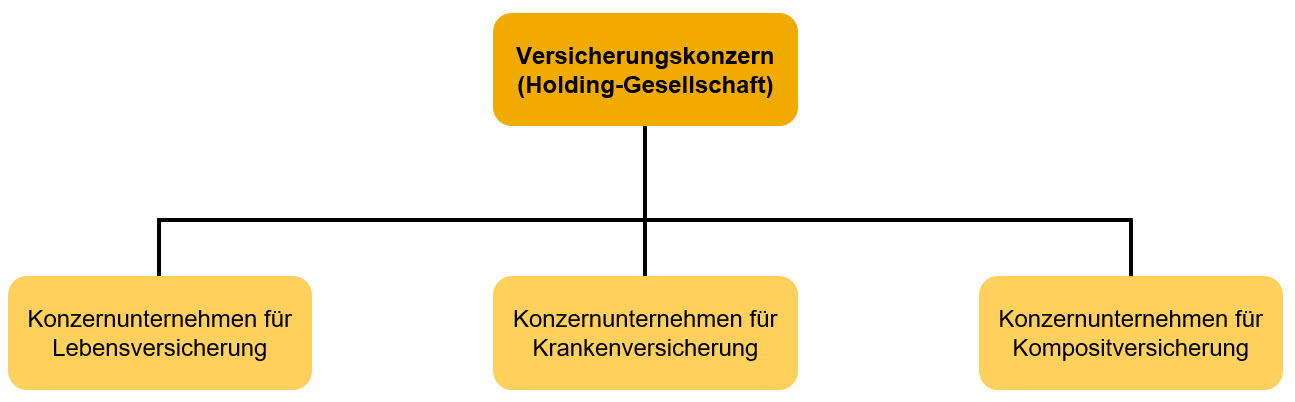
\includegraphics[width=1\textwidth]{img/Struktur_VKonzern2.jpg}
    \caption[Struktur eines Versicherungskonzerns]{Struktur eines Versicherungskonzerns\autocite{StVKonzern}}
   \label{fig:StVKonzern}
\end{figure}
\footnotetext{Vgl. eigene Darstellung angelehnt an: \cites[S. 172]{NGUYEN2013}}

%In der Praxis führt das Spartentrennungsprinzip häufig zur Bildung von größeren Mutterkonzernen, bei denen eine Holding über mehrere rechtlich selbstständige Versicherungsunternehmen verfügt (siehe Abbildung \ref{fig:StVKonzern}). Eine beispielhafte Konzernstruktur der AXA SE ist dem Anhang \ref{fig:AXAKstr} zu entnehmen. 

%\improvement{Plagiatgefahr --- bzw. Quelle prüfen oder Checken ob das in Farny auch drinnensteht}

%\hyperref[subsec:KonzernStrukturen]{4}

\subsection{Aufbau und Wettbewerb in der Kfz-Versicherungssparte}

Die Kraftfahrtversicherung ist mit einem Volumen von 29 Milliarden € in 2021 die größte Sparte in der Schadens- und Unfallversicherung in Deutschland.\autocite[Vgl.][]{GDVSUV} Zu ihr gehören die \ac{kfz}-Haftpflichtversicherung, die Fahrzeugversicherung, welche aus der Voll- und Teilkaskoversicherung besteht, sowie die Kraftfahrtunfallversicherung.\autocite[Vgl.][S. 8]{MURINGER2000}

\begin{figure}[h]
    \centering
    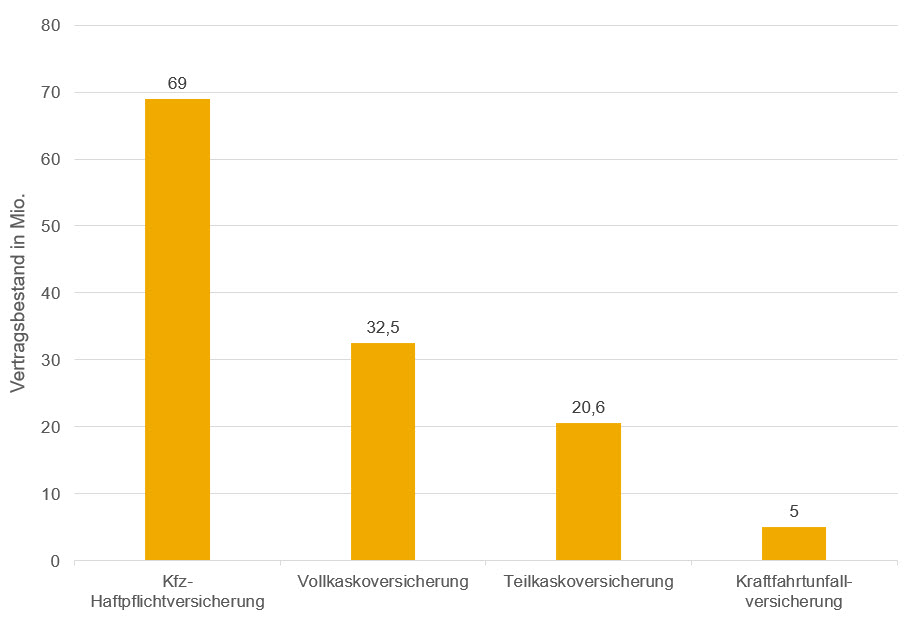
\includegraphics[width=0.9\textwidth]{img/KfzV_Bestände_an_Verträgen_2021.jpg}
    \caption[Bestände an Kfz-Versicherungsverträgen in Deutschland 2021]{Bestände an Kfz-Versicherungsverträgen in Deutschland 2021\autocite{KfzVVBestand}}
    \label{fig:KfzVVBestand}
\end{figure}
\footnotetext{Vgl. eigene Darstellung angelehnt an: GDV - Gesamtverband der Versicherer, 2022.}
%\caption[Bestände an Verträgen in der Kfz-Versicherung in Deutschland 2021]{Bestände an Verträgen in der Kfz-Versicherung in Deutschland 2021\autocite{KfzVVBestand}}
\improvement{Grafik für den Wettbewerbsfaktor: Rechte Seite: Marktanteile der Versicherungsunternehmen wie Allianz und Co.; Anzahl / Entwicklung}

Wie in Abbildung \ref{fig:KfzVVBestand} zu erkennen, macht die \ac{kfz}-Haftpflichtversicherung den größten Teil der \ac{kfz}-Versicherung aus. Der Grund dafür ist, dass eine \ac{kfz}-Zulassung in Deutschland nur mit dem Nachweis einer Haftpflichtversicherung erfolgen kann. Folglich gehört sie zu den Pflichtversicherungen und deckt den Schaden, der durch die Fahrzeugverwendung gegenüber einem Dritten entsteht. \autocite[Vgl.][S. 81]{STADLER2008}

Die Fahrzeugversicherung, welche umgangssprachlich auch als Kaskoversicherung bezeichnet wird, ist in die Fahrzeugteil- und die Fahrzeugvollversicherung untergliedert. Der wesentliche Unterschied zwischen den beiden Versicherungsarten besteht in dem Leistungsumfang. So sind bei der Fahrzeugteilversicherung ausschließlich, die durch Brand, Diebstahl, Elementarereignisse und Wildschäden verursacht wurden, gedeckt. Bei der Vollversicherung werden darüber hinaus auch Schäden abgedeckt, die durch den Versicherungsnehmer selbst verursacht werden.\autocite[Vgl.][S. 48]{FELTEN2012}

Die Kraftfahrtunfallversicherung oder auch Insassenunfallversicherung genannt, deckt im Falle eines Unfalls Personenschäden von Insassen eines Fahrzeugs ab. Versichert sind alle Unfälle, welche ausschließlich in unmittelbaren Zusammenhang mit dem Gebrauch eines Fahrzeugs entstehen, wie zum Beispiel das Fahren, Ein- und Aussteigen oder das Be- und Entladen.\autocite[Vgl.][S. 6f]{STADLER1998} 

%Dennoch werden aufgrund der großen Deckung der Leistung durch andere Versicherungen verhältnismäßig wenige Insassenunfallversicherungen abgeschlossen. So kommt bei einem fremdverschuldeten Unfall die \ac{kfz}-Haftpflichtversicherung des Unfallverursachers für alle Unfallopfer auf. Bei selbst verschuldeten Unfällen sind die Mitfahrer durch die \ac{kfz}-Haftpflichtversicherung des Fahrers bzw. des Halters abgesichert. Somit ist das Abschließen einer Insassenunfallversicherung vor allem zum Schutz des Fahrers selbst sinnvoll.\autocite[Vgl.][S. 173f]{LAMMERS2006} In der Praxis wird hierfür allerdings häufig auf Alternativen wie die private Unfallversicherung zurückgegriffen.\autocite[Vgl.][]{GRATZLA2018}  

Des Weiteren gibt es in der \ac{kfz}-Versicherungssparte einen enormen Konkurrenzdruck. So versuchen die einzelnen Anbieter insbesondere im Herbst neue Kunden zu gewinnen, da die Verträge der Versicherungsnehmer in der Regel zum 31.12 eines jeden Jahres enden und folglich bis zum 30.11 eines jeden Jahres gekündigt werden können.\autocite[Vgl.][]{WARENTEST2022} Darüber hinaus veröffentlicht der Gesamtverband der deutschen Versicherer jedes Jahr im Herbst ausgehend von der Unfallhäufigkeit der verschiedenen Fahrzeugtypen, die Preiskategorien für die einzelnen Typklassen. Daraufhin passen die meisten Versicherer ihre Beiträge an, was wiederum ihren Kunden ermöglicht, von einem Sonderkündigungsrecht Gebrauch zu machen.\autocite[Vgl.][]{NUS2022} Diese beiden Faktoren führen dazu, dass die Versicherer vor allem im Herbst versuchen, neue Kunden mit Sonderangeboten und Rabatten für sich zu gewinnen. 
%\improvement{Im Herbst: Warum im Herbst (kommt ein Tick zu spät), Verträge enden nicht sondern es gibt ein Sonderkündigungsrecht bei Preisanpassung}

Dabei sind die Kunden oftmals bereit, neben der \ac{kfz}-Versicherung weitere Policen beim gleichen Anbieter abzuschließen. Um von diesem Interesse und der Wechselbereitschaft der Kunden zu profitieren, sind die Versicherungsunternehmen bereit, kleinere Profite bis hin zu Verlusten bei der \ac{kfz}-Versicherung in Kauf zu nehmen.\autocite[Vgl.][]{HARTUNG2019} Dies lässt sich ebenfalls an der Schadensquote der \ac{kfz}-Versicherungen erkennen, welche zwischen 2015 und 2021 bei durchschnittlich 96,4 \% lag. Sie stellt das Verhältnis zwischen den Versicherungsleistungen und den Beitragseinnahmen dar.\autocite[Vgl.][]{GDVKFZ}  

%\improvement{Marktkräfte und Einflussfaktoren: Größe, D.Ö., Check24, Prozesse, vergleichsportale mit Services zum Wechseln befeuern die Wechselbereitschaft}


\newpage
